\subparagraph{Задание 4.6 (1)}

\textbf{Условие}:
Загрузить программу в отладчик (\textbf{td d:\textbackslash\/asm\textbackslash\/lab2}). Какими способами это можно сделать? Отразить способы в отчете.

\textbf{Решение}:

\begin{lstlisting}[language=Terminal]
    $ C:\td\td.exe lab2
\end{lstlisting}

Запущенный Turbo Debugger на рисунке \ref{fig:task_4_6_1__td} (стр. \pageref{fig:task_4_6_1__td}).

\begin{figure}[!htp]
    \centering
    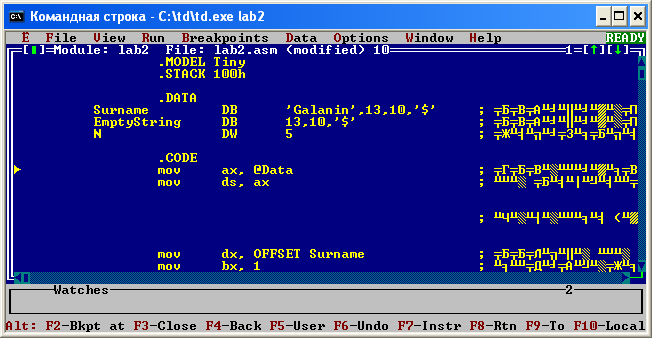
\includegraphics[width=11.2cm]
        {../_INCLUDES/task-4-6-1/td.png}
    \caption{td lab2}
    \label{fig:task_4_6_1__td}
\end{figure}

Загрузить программу в отладчик можно:
\begin{enumerate}
    \item Прописав команду \textbf{td path\textbackslash\/to\textbackslash\/file}.
    \item В программе Turbo Debugger нажать \textbf{F10}. Рисунок \ref{fig:task_4_6_1__td_file} (стр. \pageref{fig:task_4_6_1__td_file}). Нажать \textbf{влево}, выбрав пункт \textbf{File}. Нажать \textbf{Enter}. Выбираем пункт \textbf{Open}. Рисунок \ref{fig:task_4_6_1__td_file_open} (стр. \pageref{fig:task_4_6_1__td_file_open}).
\end{enumerate}

\begin{figure}[!htp]
    \centering
    \begin{minipage}{0.48\textwidth}
        \centering
        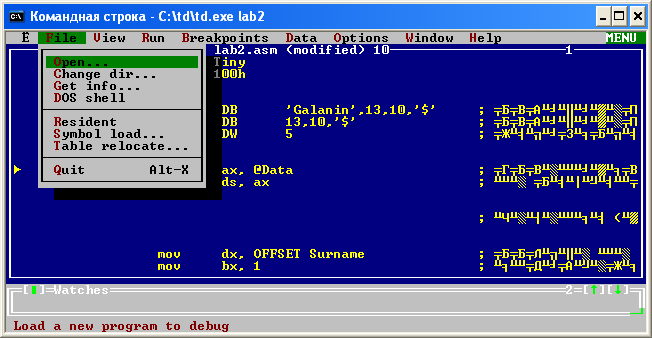
\includegraphics[width=.98\linewidth]
            {../_INCLUDES/task-4-6-1/td-file.png}
        \caption{td >\textbf{FILE}}
        \label{fig:task_4_6_1__td_file}
    \end{minipage}
    \begin {minipage}{0.48\textwidth}
        \centering
        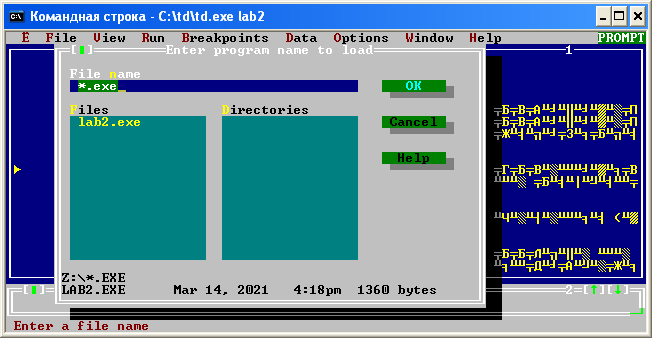
\includegraphics[width=.98\linewidth]
            {../_INCLUDES/task-4-6-1/td-file-open.png}
        \caption{td >\textbf{FILE}>\textbf{OPEN}}
        \label{fig:task_4_6_1__td_file_open}
    \end{minipage}
\end{figure}
